\documentclass[12pt,twoside]{memoir}
\usepackage{graphicx}
\usepackage[usenames]{color}
\usepackage{listings}[2000/08/23] 
\usepackage{hyperref}

% ----------------------------------------------------------
\newcommand\note[1]{\unskip\footnote{#1}}
\newcommand\foreign[1]{\emph{#1}}

\makeatletter
\newcommand\ensurecomma{\@ifnextchar,{}{\@latex@error{Don’t forget the
      comma!}{}}}
\makeatother

\newcommand\eg{\foreign{e.g.}\ensurecomma}
\newcommand\ie{\foreign{i.e.}\ensurecomma}
\newcommand\cf{\foreign{cf.\@}}

\newcommand\ensuresingleperiod{\@ifnextchar.{}{.\@}}
\newcommand\etc{\foreign{etc}\ensuresingleperiod}
\newcommand\etal{\foreign{et al}\ensuresingleperiod}
\newcommand\code[1]{\lstinline^#1^}
\newcommand\fname[1]{\texttt{#1}}

% ----------------------------------------------------------

\usepackage{exercise}

\newenvironment{Checkpoint}[1]{%
\begin{Exercise}[name={Checkpoint},title={#1}]}{%
\end{Exercise}%
\textbf{Show your work on Checkpoint~\theExercise{} to the lab monitor, %
  answering any necessary questions for them.  Have them sign before continuing.}}

\definecolor{nicered}{rgb}{.647,.129,.149}
\definecolor{listinggray}{gray}{0.9}
\definecolor{templategrey}{gray}{0.30}
\definecolor{commandlinebackground}{gray}{0.25}
\definecolor{commandlineforeground}{gray}{0.85}
\definecolor{commandpromptforeground}{gray}{0.55}


\DeclareGraphicsExtensions{.eps,.pdf,.png,.gif,.jpg}


% ---------- listing code parameters
\lstset{language=java,
  basicstyle=\small\ttfamily,
  numbers=none, 
  numberstyle=\tiny, 
  stepnumber=1, 
  numbersep=5pt,
  frame=single,
  captionpos=b,
  rulecolor=\color{nicered}
}

% ----- Command-line listing language
\lstdefinelanguage{cline}
{
  morecomment=[s][\color{commandpromptforeground}]{\~}{\%},
}

% ----- Command-line environment 
\lstnewenvironment{commandline}[1][]
  {\lstset{language=cline,numbers=none,frame=none,backgroundcolor=\color{commandlinebackground},basicstyle=\color{commandlineforeground},nolol,#1}}
  {}

\newcommand{\artDir}{../art}
\newcommand{\lab}[1]{%
\title{CIS 201 Computer Science I\\Fall 2009 Lab #1}%
\maketitle%
}

\setlength{\hoffset}{0in}
\setlength{\voffset}{0in}
\settypeblocksize{9in}{6.5in}{*}
\setlrmargins{*}{*}{1}
\setulmargins{*}{*}{*}
\setheadfoot{\onelineskip}{2\onelineskip}
\checkandfixthelayout

\begin{document}
\lab{06}

\begin{itemize}
\item Build a solution with multiple classes.
\item Create new instances of your class and use them in a game.
\item Create a class which has state (and implement getter and setter
  methods). 
\end{itemize}

\begin{figure}[htb]
  \begin{center}    
    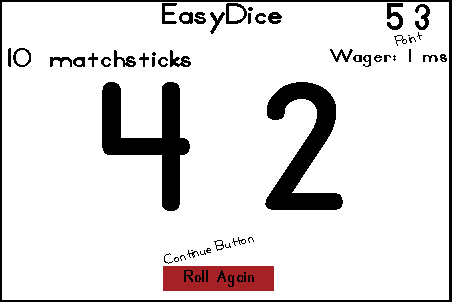
\includegraphics[width=6in]{\artDir/easyDiceStringSprite-design}  
    \caption{EasyDice Design}
  \label{fig:login}
  \end{center}
\end{figure}

\begin{Checkpoint}{Getting Started}
  Create a directory, \fname{Lab06} in your CS1 directory. Copy
  \fname{EasyDice.java}  and \fname{EasyButton.java} (location:
  \url{/home/student/Classes/201/Labs/06/EasyDice.java} \url{/home/student/Classes/201/Labs/06/EasyButton.java}) into the new
  lab directory.

  \fname{EasyDice.java} contains a complete game. Take a look at the
  code and you will find that one class, \code{OneDie}, does not
  exist. Your job is to design and build that class so that
  \code{EasyDice} can be played.

  Create a new, empty class called \code{OneDie}. The class
  \code{extends} \code{StringSprite}. It must be in the lab directory
  (the same directory as \code{EasyDice}). 

  Insert a properly formatted header comment for the \code{OneDie}
  class and include both author's names.

  Examine the \code{EasyDice} code. In the header comment for
  \code{OneDie}, note each \code{OneDie} method called by
  \code{EasyDice}. Deduce as much of the method header as you can for
  each one. (Don't forget the \emph{constructor}; it is a method,
  too.)
\end{Checkpoint}

\begin{Checkpoint}{Implement Stubs}
  Compare your list of methods of \code{OneDie} with the documentation
  for \code{StringSprite} and divide the list in two: those methods
  already defined in \code{StringSprite} and those that are not. You
  get all the methods in the first list by extending
  \code{StringSprite}; you must define the ones in the second list.

  A ``stub'' is a method that doesn't actually do anything. It is used
  to permit code to compile while you actually work on getting the
  code to function. The stub of a \code{void} method (or a
  constructor) is easy: it is empty. There is no need to return any
  value since none is expected.

  A stub for a method that returns a value just returns some
  value. For \code{boolean} you can just return \code{false} and for
  \code{int} you can just return some number in the expected
  range. You could do the same for \code{double} or \code{char}. Stubs
  that are supposed to return objects are a bit trickier but you don't
  have any of those here.

  Put stubs for all your functions into the \code{OneDie} class and
  get \code{EasyDice} to compile. You can run it, too, and you won't
  see much.
\end{Checkpoint}

\begin{Checkpoint}{Add State}
  The big extension of \code{OneDie} over \code{StringSprite} is that
  the die has a face value. Add a field to hold the value.

  Add comments to the getter and setter methods for the die's face
  value. Also modify them so that they interact with the state you
  added. 

  Modify the setter so that the displayed text of \code{OneDie} is
  updated if the value is changed. Also make sure that the face value
  of the die is only changed if the number is in the range [1-6].

  Why would you worry about an out of range face value? 
\end{Checkpoint}

\begin{Checkpoint}{Roll the Dice}
  The roll method of \code{OneDie} must pick a random integer on the
  range [1-6]. How do we get a random number?

  If you said ``Call \code{randomInt},'' give yourself a cookie. There
  is a problem: \code{StringSprite} does not have a \code{randomInt}
  method. That method is defined in the \code{Game} class.

  How can we get the currently running game object? It is not enough
  to get the \code{Game} class; we need an actual \code{Game}
  object. What to do... \code{Game.getCurrentGame()} is a method
  defined for the \code{Game} class which returns a reference to the
  current game. We can use it to call \code{randomInt} (what
  parameters do you pass to \code{randomInt} to get numbers on the
  range [1-6]?). 

  Write \code{roll} so that it rolls \code{OneDie}. 

  Compile, run, and play a little bit of the game (to convince
  yourself that it works). 

  Be prepared to explain the line which calls \code{randomInt}, both
  the parameter(s) and the \code{Game.getCurrentGame()} part.
\end{Checkpoint}

\Large{Log off of the lab computer you are using before leaving they
  lab. Anyone entering the lab has unlimited access to your files if
  you remain logged on. \textbf{DO NOT} turn off lab computers! They
  are a shared resource and there might be someone else logged in to
  ``your'' machine.}

\Large{Clean up your work area, push in the chair, and have a good
  week.}

\end{document}
